
% 数学格式

%表示角度的圆圈直接用° (搜狗打du即可)
%\newcommand{\abs}[1]{\left\lvert#1 \right\rvert} %定义绝对值 % physics 宏包已有
\newcommand{\D}{\,\mathrm{d}} %微分算符正体
\newcommand{\I}{\mathrm{i}} %虚数单位正体
\newcommand{\E}{\mathrm{e}} %自然对数底整体
\renewcommand{\vec}[1]{\boldsymbol{\mathbf{#1}}}%矢量用正体加粗字母, 大写也可以(电场) %只用 mathbf 对希腊字母没用
\newcommand{\mat}[1]{\boldsymbol{\mathbf{#1}}}   %矩阵用正体加粗字母, 小写也可以(泡力矩阵)
\newcommand{\ten}[1]{\boldsymbol{\mathbf{#1}}} % 张量与矩阵相同
\newcommand{\Nabla}{\vec\nabla}
\renewcommand{\Tr}{^{\textup{T}}} %矩阵转置 % 覆盖 physics 宏包的 Trace
\newcommand{\uvec}[1]{\hat{\boldsymbol{\mathbf{#1}}}} %单位矢量为黑体加 hat
\renewcommand{\pmat}[1]{\begin{pmatrix}#1\end{pmatrix}} % 矩阵圆括号, 覆盖 physics 宏包 (pauli matrix)
\newcommand{\ali}[1]{\begin{aligned}#1\end{aligned}}
\newcommand{\leftgroup}[1]{\left\{\begin{aligned}#1\end{aligned}\right.}
\newcommand{\vmat}[1]{\begin{vmatrix}#1\end{vmatrix}} % 行列式
\newcommand{\Cj}{^*} % 复共轭
\newcommand{\dfracH}{\rule[-0.5cm]{0pt}{1.3cm}} % 全尺寸分数 dfrac 在表格中的高度
\newcommand{\Her}{^\dag} %厄米共轭
\newcommand{\Q}[1]{\hat #1}
\newcommand{\sinc}{\mathrm{sinc}} % sinc 函数
\newcommand{\Si}[1]{\ \si{#1}} % 国际单位
\newcommand{\x}{\texttt} % 代码字体
\newcommand{\bb}{\textbf} % 粗体
\newcommand{\les}{\leqslant} % 小于等于号
\newcommand{\ges}{\geqslant} % 大于等于号

% 设置 Matlab 格式,用于MatlabStyle.tex
\usepackage{color} %red, green, blue, yellow, cyan, magenta, black, white
\definecolor{mygreen}{RGB}{28,172,0}
\definecolor{mylilas}{RGB}{170,55,241}
\definecolor{string}{RGB}{160,32,240}
\definecolor{comment}{RGB}{34,139,34}
\definecolor{warning}{RGB}{255,100,0}
\definecolor{error}{RGB}{230,0,0}

% 其他
\newcommand{\entry}[2]{\section{#1}\label{#2}\input{./contents/#2}}% 主程序中使用,从 contents 文件夹加入词条
\newcommand{\Entry}[2]{\section{#1}\label{#2}\input{./contents1/#2}}% 从 contents1 中加入词条(contents1 里面用于存放超出力学分册的内容)
\newcommand{\pentry}[1]{\begin{mdframed}\bb{预备知识\ } #1 \end{mdframed}}%预备知识的格式
\newcommand{\rentry}[1]{\begin{mdframed}\bb{拓展阅读\ } #1 \end{mdframed}}%拓展阅读的格式
\newcommand{\eentry}[1]{\begin{mdframed}\bb{应用举例\ } #1 \end{mdframed}}%应用举例的格式

% 图片的格式
%\newcommand{\fig}[3]{\begin{figure}[ht]\centering\includegraphics[width= #2]{./figures/#1.pdf}\caption{#3}\end{figure}}
% 控制行代码环境(注意不能用于段落最后!)
% zihao 命令,小N号用 -N,大N号用 +N
\newenvironment{Command}{\vspace{0.2cm} \\ \ttfamily\zihao{5}}{\vspace{0.2cm}\\}

% 淘宝模板其他设置
\mdfsetup{%
frametitlealignment=\noindent\raggedright,
middlelinecolor=gray,
middlelinewidth=.3pt,
backgroundcolor=white,
roundcorner=6pt}
%-------------------------------------------------------------------------------
% Colors adapted from Material Design
%-------------------------------------------------------------------------------

% Red
\definecolor{red-50}{RGB}{255,235,238}
\definecolor{red-100}{RGB}{255,205,210}
\definecolor{red-200}{RGB}{239,154,154}
\definecolor{red-300}{RGB}{229,115,115}
\definecolor{red-400}{RGB}{239,83,80}
\definecolor{red-500}{RGB}{244,67,54}
\definecolor{red-600}{RGB}{229,57,53}
\definecolor{red-700}{RGB}{211,47,47}
\definecolor{red-800}{RGB}{198,40,40}
\definecolor{red-900}{RGB}{183,28,28}
\definecolor{red-A100}{RGB}{255,138,128}
\definecolor{red-A200}{RGB}{255,82,82}
\definecolor{red-A400}{RGB}{255,23,68}
\definecolor{red-A700}{RGB}{213,0,0}

% Pink
\definecolor{pink-50}{RGB}{252,228,236}
\definecolor{pink-100}{RGB}{248,187,208}
\definecolor{pink-200}{RGB}{244,143,177}
\definecolor{pink-300}{RGB}{240,98,146}
\definecolor{pink-400}{RGB}{236,64,122}
\definecolor{pink-500}{RGB}{233,30,99}
\definecolor{pink-600}{RGB}{216,27,96}
\definecolor{pink-700}{RGB}{194,24,91}
\definecolor{pink-800}{RGB}{173,20,87}
\definecolor{pink-900}{RGB}{136,14,79}
\definecolor{pink-A100}{RGB}{255,128,171}
\definecolor{pink-A200}{RGB}{255,64,129}
\definecolor{pink-A400}{RGB}{245,0,87}
\definecolor{pink-A700}{RGB}{197,17,98}

% Purple
\definecolor{purple-50}{RGB}{243,229,245}
\definecolor{purple-100}{RGB}{225,190,231}
\definecolor{purple-200}{RGB}{206,147,216}
\definecolor{purple-300}{RGB}{186,104,200}
\definecolor{purple-400}{RGB}{171,71,188}
\definecolor{purple-500}{RGB}{156,39,176}
\definecolor{purple-600}{RGB}{142,36,170}
\definecolor{purple-700}{RGB}{123,31,162}
\definecolor{purple-800}{RGB}{106,27,154}
\definecolor{purple-900}{RGB}{74,20,140}
\definecolor{purple-A100}{RGB}{234,128,252}
\definecolor{purple-A200}{RGB}{224,64,251}
\definecolor{purple-A400}{RGB}{213,0,249}
\definecolor{purple-A700}{RGB}{170,0,255}

% Deep-Purple
\definecolor{deep-purple-50}{RGB}{237,231,246}
\definecolor{deep-purple-100}{RGB}{209,196,233}
\definecolor{deep-purple-200}{RGB}{179,157,219}
\definecolor{deep-purple-300}{RGB}{149,117,205}
\definecolor{deep-purple-400}{RGB}{126,87,194}
\definecolor{deep-purple-500}{RGB}{103,58,183}
\definecolor{deep-purple-600}{RGB}{94,53,177}
\definecolor{deep-purple-700}{RGB}{81,45,168}
\definecolor{deep-purple-800}{RGB}{69,39,160}
\definecolor{deep-purple-900}{RGB}{49,27,146}
\definecolor{deep-purple-A100}{RGB}{179,136,255}
\definecolor{deep-purple-A200}{RGB}{124,77,255}
\definecolor{deep-purple-A400}{RGB}{101,31,255}
\definecolor{deep-purple-A700}{RGB}{98,0,234}

% Indigo
\definecolor{indigo-50}{RGB}{232,234,246}
\definecolor{indigo-100}{RGB}{197,202,233}
\definecolor{indigo-200}{RGB}{159,168,218}
\definecolor{indigo-300}{RGB}{121,134,203}
\definecolor{indigo-400}{RGB}{92,107,192}
\definecolor{indigo-500}{RGB}{63,81,181}
\definecolor{indigo-600}{RGB}{57,73,171}
\definecolor{indigo-700}{RGB}{48,63,159}
\definecolor{indigo-800}{RGB}{40,53,147}
\definecolor{indigo-900}{RGB}{26,35,126}
\definecolor{indigo-A100}{RGB}{140,158,255}
\definecolor{indigo-A200}{RGB}{83,109,254}
\definecolor{indigo-A400}{RGB}{61,90,254}
\definecolor{indigo-A700}{RGB}{48,79,254}

% Blue
\definecolor{blue-50}{RGB}{227,242,253}
\definecolor{blue-100}{RGB}{187,222,251}
\definecolor{blue-200}{RGB}{144,202,249}
\definecolor{blue-300}{RGB}{100,181,246}
\definecolor{blue-400}{RGB}{66,165,245}
\definecolor{blue-500}{RGB}{33,150,243}
\definecolor{blue-600}{RGB}{30,136,229}
\definecolor{blue-700}{RGB}{25,118,210}
\definecolor{blue-800}{RGB}{21,101,192}
\definecolor{blue-900}{RGB}{13,71,161}
\definecolor{blue-A100}{RGB}{130,177,255}
\definecolor{blue-A200}{RGB}{68,138,255}
\definecolor{blue-A400}{RGB}{41,121,255}
\definecolor{blue-A700}{RGB}{41,98,255}

% Light-blue
\definecolor{light-blue-50}{RGB}{225,245,254}
\definecolor{light-blue-100}{RGB}{179,229,252}
\definecolor{light-blue-200}{RGB}{129,212,250}
\definecolor{light-blue-300}{RGB}{79,195,247}
\definecolor{light-blue-400}{RGB}{41,182,246}
\definecolor{light-blue-500}{RGB}{3,169,244}
\definecolor{light-blue-600}{RGB}{3,155,229}
\definecolor{light-blue-700}{RGB}{2,136,209}
\definecolor{light-blue-800}{RGB}{2,119,189}
\definecolor{light-blue-900}{RGB}{1,87,155}
\definecolor{light-blue-A100}{RGB}{128,216,255}
\definecolor{light-blue-A200}{RGB}{64,196,255}
\definecolor{light-blue-A400}{RGB}{0,176,255}
\definecolor{light-blue-A700}{RGB}{0,145,234}

% Cyan
\definecolor{cyan-50}{RGB}{224,247,250}
\definecolor{cyan-100}{RGB}{178,235,242}
\definecolor{cyan-200}{RGB}{128,222,234}
\definecolor{cyan-300}{RGB}{77,208,225}
\definecolor{cyan-400}{RGB}{38,198,218}
\definecolor{cyan-500}{RGB}{0,188,212}
\definecolor{cyan-600}{RGB}{0,172,193}
\definecolor{cyan-700}{RGB}{0,151,167}
\definecolor{cyan-800}{RGB}{0,131,143}
\definecolor{cyan-900}{RGB}{0,96,100}
\definecolor{cyan-A100}{RGB}{132,255,255}
\definecolor{cyan-A200}{RGB}{24,255,255}
\definecolor{cyan-A400}{RGB}{0,229,255}
\definecolor{cyan-A700}{RGB}{0,184,212}

% Teal
\definecolor{teal-50}{RGB}{224,242,241}
\definecolor{teal-100}{RGB}{178,223,219}
\definecolor{teal-200}{RGB}{128,203,196}
\definecolor{teal-300}{RGB}{77,182,172}
\definecolor{teal-400}{RGB}{38,166,154}
\definecolor{teal-500}{RGB}{0,150,136}
\definecolor{teal-600}{RGB}{0,137,123}
\definecolor{teal-700}{RGB}{0,121,107}
\definecolor{teal-800}{RGB}{0,105,92}
\definecolor{teal-900}{RGB}{0,77,64}
\definecolor{teal-A100}{RGB}{167,255,235}
\definecolor{teal-A200}{RGB}{100,255,218}
\definecolor{teal-A400}{RGB}{29,233,182}
\definecolor{teal-A700}{RGB}{0,191,165}

% Green
\definecolor{green-50}{RGB}{232,245,233}
\definecolor{green-100}{RGB}{200,230,201}
\definecolor{green-200}{RGB}{165,214,167}
\definecolor{green-300}{RGB}{129,199,132}
\definecolor{green-400}{RGB}{102,187,106}
\definecolor{green-500}{RGB}{76,175,80}
\definecolor{green-600}{RGB}{67,160,71}
\definecolor{green-700}{RGB}{56,142,60}
\definecolor{green-800}{RGB}{46,125,50}
\definecolor{green-900}{RGB}{27,94,32}
\definecolor{green-A100}{RGB}{185,246,202}
\definecolor{green-A200}{RGB}{105,240,174}
\definecolor{green-A400}{RGB}{0,230,118}
\definecolor{green-A700}{RGB}{0,200,83}

% Light-green
\definecolor{light-green-50}{RGB}{241,248,233}
\definecolor{light-green-100}{RGB}{220,237,200}
\definecolor{light-green-200}{RGB}{197,225,165}
\definecolor{light-green-300}{RGB}{174,213,129}
\definecolor{light-green-400}{RGB}{156,204,101}
\definecolor{light-green-500}{RGB}{139,195,74}
\definecolor{light-green-600}{RGB}{124,179,66}
\definecolor{light-green-700}{RGB}{104,159,56}
\definecolor{light-green-800}{RGB}{85,139,47}
\definecolor{light-green-900}{RGB}{51,105,30}
\definecolor{light-green-A100}{RGB}{204,255,144}
\definecolor{light-green-A200}{RGB}{178,255,89}
\definecolor{light-green-A400}{RGB}{118,255,3}
\definecolor{light-green-A700}{RGB}{100,221,23}

% Lime
\definecolor{lime-50}{RGB}{249,251,231}
\definecolor{lime-100}{RGB}{240,244,195}
\definecolor{lime-200}{RGB}{230,238,156}
\definecolor{lime-300}{RGB}{220,231,117}
\definecolor{lime-400}{RGB}{212,225,87}
\definecolor{lime-500}{RGB}{205,220,57}
\definecolor{lime-600}{RGB}{192,202,51}
\definecolor{lime-700}{RGB}{175,180,43}
\definecolor{lime-800}{RGB}{158,157,36}
\definecolor{lime-900}{RGB}{130,119,23}
\definecolor{lime-A100}{RGB}{244,255,129}
\definecolor{lime-A200}{RGB}{238,255,65}
\definecolor{lime-A400}{RGB}{198,255,0}
\definecolor{lime-A700}{RGB}{174,234,0}

% Yellow
\definecolor{yellow-50}{RGB}{255,253,231}
\definecolor{yellow-100}{RGB}{255,249,196}
\definecolor{yellow-200}{RGB}{255,245,157}
\definecolor{yellow-300}{RGB}{255,241,118}
\definecolor{yellow-400}{RGB}{255,238,88}
\definecolor{yellow-500}{RGB}{255,235,59}
\definecolor{yellow-600}{RGB}{253,216,53}
\definecolor{yellow-700}{RGB}{251,192,45}
\definecolor{yellow-800}{RGB}{249,168,37}
\definecolor{yellow-900}{RGB}{245,127,23}
\definecolor{yellow-A100}{RGB}{255,255,141}
\definecolor{yellow-A200}{RGB}{255,255,0}
\definecolor{yellow-A400}{RGB}{255,234,0}
\definecolor{yellow-A700}{RGB}{255,214,0}

% Amber
\definecolor{amber-50}{RGB}{255,248,225}
\definecolor{amber-100}{RGB}{255,236,179}
\definecolor{amber-200}{RGB}{255,224,130}
\definecolor{amber-300}{RGB}{255,213,79}
\definecolor{amber-400}{RGB}{255,202,40}
\definecolor{amber-500}{RGB}{255,193,7}
\definecolor{amber-600}{RGB}{255,179,0}
\definecolor{amber-700}{RGB}{255,160,0}
\definecolor{amber-800}{RGB}{255,143,0}
\definecolor{amber-900}{RGB}{255,111,0}
\definecolor{amber-A100}{RGB}{255,229,127}
\definecolor{amber-A200}{RGB}{255,215,64}
\definecolor{amber-A400}{RGB}{255,196,0}
\definecolor{amber-A700}{RGB}{255,171,0}

% Orange
\definecolor{orange-50}{RGB}{255,243,224}
\definecolor{orange-100}{RGB}{255,224,178}
\definecolor{orange-200}{RGB}{255,204,128}
\definecolor{orange-300}{RGB}{255,183,77}
\definecolor{orange-400}{RGB}{255,167,38}
\definecolor{orange-500}{RGB}{255,152,0}
\definecolor{orange-600}{RGB}{251,140,0}
\definecolor{orange-700}{RGB}{245,124,0}
\definecolor{orange-800}{RGB}{239,108,0}
\definecolor{orange-900}{RGB}{230,81,0}
\definecolor{orange-A100}{RGB}{255,209,128}
\definecolor{orange-A200}{RGB}{255,171,64}
\definecolor{orange-A400}{RGB}{255,145,0}
\definecolor{orange-A700}{RGB}{255,109,0}

% Deep-orange
\definecolor{deep-orange-50}{RGB}{251,233,231}
\definecolor{deep-orange-100}{RGB}{255,204,188}
\definecolor{deep-orange-200}{RGB}{255,171,145}
\definecolor{deep-orange-300}{RGB}{255,138,101}
\definecolor{deep-orange-400}{RGB}{255,112,67}
\definecolor{deep-orange-500}{RGB}{255,87,34}
\definecolor{deep-orange-600}{RGB}{244,81,30}
\definecolor{deep-orange-700}{RGB}{230,74,25}
\definecolor{deep-orange-800}{RGB}{216,67,21}
\definecolor{deep-orange-900}{RGB}{191,54,12}
\definecolor{deep-orange-A100}{RGB}{255,158,128}
\definecolor{deep-orange-A200}{RGB}{255,110,64}
\definecolor{deep-orange-A400}{RGB}{255,61,0}
\definecolor{deep-orange-A700}{RGB}{221,44,0}

% Brown
\definecolor{brown-50}{RGB}{239,235,233}
\definecolor{brown-100}{RGB}{215,204,200}
\definecolor{brown-200}{RGB}{188,170,164}
\definecolor{brown-300}{RGB}{161,136,127}
\definecolor{brown-400}{RGB}{141,110,99}
\definecolor{brown-500}{RGB}{121,85,72}
\definecolor{brown-600}{RGB}{109,76,65}
\definecolor{brown-700}{RGB}{93,64,55}
\definecolor{brown-800}{RGB}{78,52,46}
\definecolor{brown-900}{RGB}{62,39,35}

% Grey
\definecolor{grey-50}{RGB}{250,250,250}
\definecolor{grey-100}{RGB}{245,245,245}
\definecolor{grey-200}{RGB}{238,238,238}
\definecolor{grey-300}{RGB}{224,224,224}
\definecolor{grey-400}{RGB}{189,189,189}
\definecolor{grey-500}{RGB}{158,158,158}
\definecolor{grey-600}{RGB}{117,117,117}
\definecolor{grey-700}{RGB}{97,97,97}
\definecolor{grey-800}{RGB}{66,66,66}
\definecolor{grey-900}{RGB}{33,33,33}

% Blue-grey
\definecolor{blue-grey-50}{RGB}{236,239,241}
\definecolor{blue-grey-100}{RGB}{207,216,220}
\definecolor{blue-grey-200}{RGB}{176,190,197}
\definecolor{blue-grey-300}{RGB}{144,164,174}
\definecolor{blue-grey-400}{RGB}{120,144,156}
\definecolor{blue-grey-500}{RGB}{96,125,139}
\definecolor{blue-grey-600}{RGB}{84,110,122}
\definecolor{blue-grey-700}{RGB}{69,90,100}
\definecolor{blue-grey-800}{RGB}{55,71,79}
\definecolor{blue-grey-900}{RGB}{38,50,56}

\definecolor{black}{RGB}{0,0,0}
\definecolor{white}{RGB}{255,255,255}

\usepackage{xeCJK}
\usepackage[papersize={185mm,260mm},hmargin=2.1cm,vmargin=1in]{geometry}
%%%%%%%%%%%%% 有需要可以自行调用字体
\setCJKmainfont
  [ItalicFont=KaiTi,
  BoldFont=SimHei]
  {SimSun}
\setCJKsansfont{SimHei}
\renewcommand{\heiti}
  {\CJKfontspec{SimHei}}
\renewcommand{\kaishu}
  {\CJKfontspec{KaiTi}}
\renewcommand{\youyuan}
  % {\CJKfontspec{YouYuan}}
% \renewcommand{\fangsong}
  % {\CJKfontspec{FangSong}}

\setmainfont{Times New Roman}
\setsansfont{Arial}
%%%%%%%%%%%%%%%%%%%%%%%%%%%
\usepackage{titletoc}
\usepackage{titlesec}
\titleformat{\section}[display]% 词条格式 (section)
{\zihao{4}\color{deep-orange-A700}\filright\kaishu\sf}
{}{.5em}{}[\color{orange-A700}\vspace*{-1.2em}\rule{\textwidth}{2pt}] %在节上显示*号

\definecolor{myblue}{RGB}{10,10,180} % 用于 subtitle
\titleformat{\subsection}[hang] % 小标题格式 (subsection)
{\normalsize\color{myblue}\heiti\filright} % 颜色和字体
{} % label
{0.5cm} % 小标题下方空白
{\vspace*{-0.2cm}\\} % 小标题前的命令
%[]  % 小标题下方文字结束后下方的命令

\titlespacing*{\section}
{0em}{1.5ex plus .1ex minus .2ex}{.5ex minus .1ex}
%\contentsmargin{0pt}
\titlecontents{part}[3.5em]{\vspace{1.25\baselineskip}\centering\heiti\zihao{3}}{\contentslabel{3.6em}}{\hspace*{-3.6em}}
        {\hfill}
\titlecontents{chapter}[5em]{\vspace{0.55\baselineskip}\fontsize{13.05pt}{16pt}\selectfont\heiti}{\contentslabel{4.5em}}{\hspace*{-4.5em}}
        {\hspace{.5em}}[\titlerule]
\titlecontents*{section}[0pc]
  {\addvspace{3pt}\zihao{-4}}
  {}
  {}
  {\,\textsuperscript{\color{blue-A700}[\thecontentspage]}}[\quad]

\titlecontents*{subsection}[1.8pc]
  {\zihao{5}}
  {\thecontentslabel. }
  {}
  {, \thecontentspage}
  [.---][.]
\titlespacing*{\subsection} {0pt}{1.25ex plus 1ex minus .2ex}{.5ex plus .2ex}

\usepackage{tikz}
\usepackage{multicol}


\newtheoremstyle{mystyle}{8pt}{8pt}{}{}{\bfseries}{}{\newline}
{\thmname{#1}\thmnumber{ #2}\thmnote{\bf #3}\indent}  % 新增:最后一个{}
\theoremstyle{mystyle}
\newtheorem{example}{\normalsize{例}}
\newtheorem{Thm}{\normalsize{{定理}}}
\newtheorem*{slove}{\normalsize{{【解】}}} % * 表示不编号!


\usepackage{indentfirst}
\usepackage[pdfstartview=FitH,
            CJKbookmarks=true,
            bookmarksnumbered=false,
            bookmarksopen=true,
            linktocpage=true,
            colorlinks, %注释掉此项则交叉引用为彩色边框(将colorlinks和pdfborder同时注释掉)
            pdfborder=001,   %注释掉此项则交叉引用为彩色边框
            linkcolor=blue-A700,
            anchorcolor=blue-A700,
            citecolor=blue-A700]{hyperref}
\setlength{\abovecaptionskip}{0pt}
\setlength{\belowcaptionskip}{3pt}

\newcommand\upref[1]{\textsuperscript{[\pageref{#1}]}}
\renewcommand\sectionmark[1]{%
\markright{\leftmark}}
\renewcommand{\textfraction}{0.05}
\renewcommand{\topfraction}{0.95}
\renewcommand{\bottomfraction}{0.65}
\renewcommand{\floatpagefraction}{0.60}
\makeatletter
\setlength{\@fptop}{5pt}
\setlength{\floatsep}{10pt \@plus3pt \@minus1pt}
\setlength{\intextsep}{12pt \@plus3pt \@minus2pt}
\setlength{\textfloatsep}{10pt \@plus3pt \@minus2pt}
\def\@makechapterhead#1{%
  \null\vskip3.8cm\@tempskipa = \glueexpr \CTEX@chapter@beforeskip \relax
  \ifodd \CTEX@chapter@fixbeforeskip
    \CTEX@fixbeforeskip
  \fi
  \vspace*{\@tempskipa}%
  {\normalfont \parindent \dimexpr \CTEX@chapter@indent \relax
   \CTEX@chapter@format\centering
   \ifnum \c@secnumdepth >\m@ne
     \if@mainmatter
       \ifodd \CTEX@chapter@numbering
         \CTEX@chaptername \CTEX@chapter@aftername
       \fi
     \fi
   \fi
   \par\vskip18pt%
   \CTEX@chapter@titleformat{#1}%
   \CTEX@chapter@aftertitle
   \nobreak
   \vfill\vskip \glueexpr \CTEX@chapter@afterskip \relax
   \newpage
  }}
\def\@makeschapterhead#1{%
  \null\vskip-2.8cm\@tempskipa = \glueexpr \CTEX@chapter@beforeskip \relax
  \ifodd \CTEX@chapter@fixbeforeskip
    \CTEX@fixbeforeskip
  \fi
  \vspace*{\@tempskipa}%
  {\normalfont \parindent \dimexpr \CTEX@chapter@indent \relax
   \CTEX@chapter@format
   \interlinepenalty\@M
   \CTEX@chapter@titleformat{#1}
   \CTEX@chapter@aftertitle
   \nobreak
   \null\vskip-2cm
   \vskip \glueexpr \CTEX@chapter@afterskip \relax
  }}
\makeatother

% 新增:以下命令为新加
\makeatletter
\def\HyRef@autopageref#1{%
 \hyperref[{#1}]{[\pageref*{#1}]}%
}
\makeatother

\renewcommand{\equationautorefname}{式}
\renewcommand{\figureautorefname}{图}
\renewcommand{\tableautorefname}{表}
\newcommand{\Exaautorefname}{例}
\newcommand{\exampleautorefname}{例}

\makeatletter
\def\thmt@amsthmlistbreakhack{%
  \leavevmode
  \vspace{-\baselineskip}%
  \par
  \everypar{\setbox\z@\lastbox\everypar{}}%
}
\makeatother

%\let\eqref\autoref
\newcommand{\exref}[1]{\autoref{#1}}
\renewcommand\upref[1]{\textsuperscript{\autopageref{#1}}}

%\AtBeginEnvironment{example}{\normalsize} % 调整 example 环境字号(标题也会受影响!不能用!),不能调整字体! 以下定义 exam 环境,以后一律使用 exam 环境!
\newenvironment{exam}[1]{\begin{example}[\;\; #1]\kaishu\hspace*{1.7em}}{\end{example}} % 调整字体字号

% 新增结束

% 编号在每个 section 内从 1 开始
\numberwithin{equation}{section}
\renewcommand\theequation{\arabic{equation}}
\numberwithin{example}{section}
\renewcommand\theexample{\arabic{example}}
\numberwithin{figure}{section}
\renewcommand\thefigure{\arabic{figure}}
\numberwithin{table}{section}
\renewcommand\thetable{\arabic{table}}
\numberwithin{chapter}{part}


\begin{document}
\renewcommand{\thelstlisting}{\arabic{lstlisting}}
\lstset{language=Matlab,
    basicstyle= \ttfamily, % 变量以外的符号
    breaklines=true,%?  
    keywordstyle=\color{blue},% 关键字的颜色
    morekeywords=[2]{1}, keywordstyle=[2]{\color{black}}, %? 
    identifierstyle=\color{black},%? 
    stringstyle=\color{string}, % 字符串的颜色
    commentstyle=\color{comment},% 注释的格式
    showstringspaces=false,% 不显示空格符
    numbers=left,
    numberstyle={\tiny \color{gray}}, % 行号大小
    numbersep=11pt, % 行号距离
    %backgroundcolor=\color{yellow}, % 背景颜色
    emph=[1]{for,end,break},emphstyle=[1]\color{blue} % 指定单词高量
    %morekeywords={smooth} % 增加 keywords
     % 删除 keywords
}

% Matlab 代码环境
\newcommand{\Matlab}{\begin{lstlisting}[language=Matlab, deletekeywords={rand, disp, error, nargin, flipud, fliplr, plot, axis, hold, roots, linspace, figure, title, sign, find, zeros, fzero, exp, format, sin, cos, tan, cot, asin, acos, atan, real, imag, sum, mean, diff, floor, ceil, sinh, cosh, tanh, round, ans, size, randn, eye, magic}]} % 设置 Matlab 颜色
\begin{titlepage}

\includepdf{./figures/frontcover.pdf}
\newpage
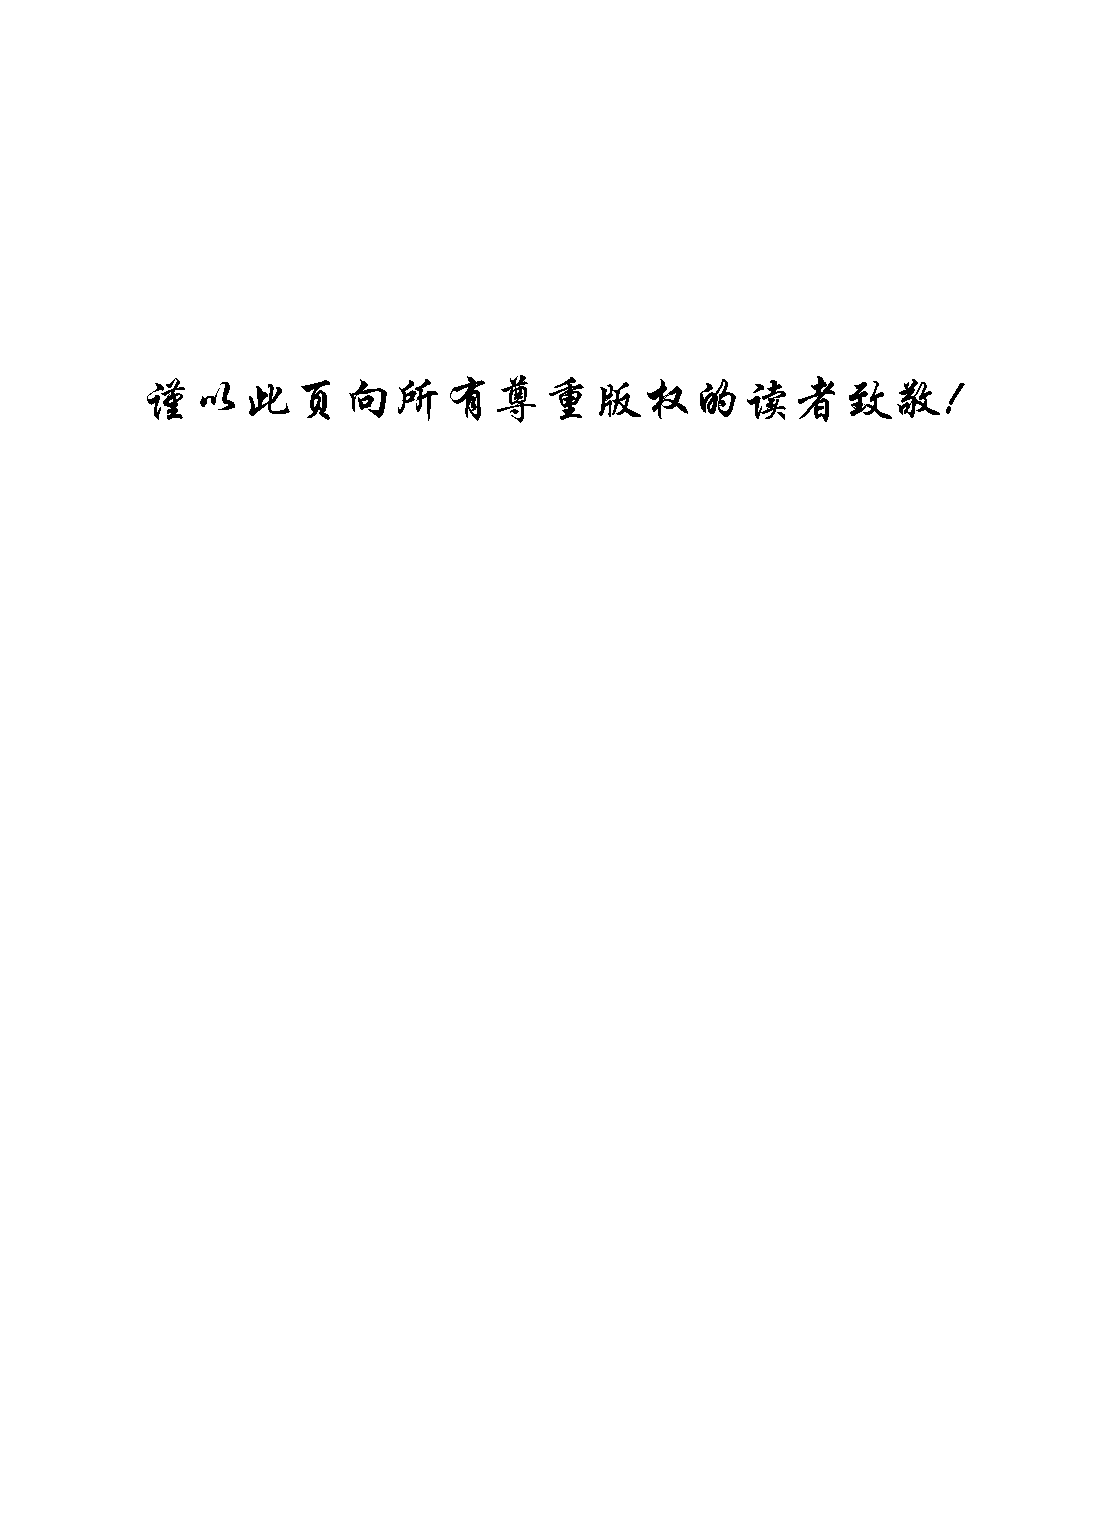
\includepdf{./figures/dedication.pdf}
\end{titlepage}
\frontmatter % 开始罗马数字页码
% 版权声明 关于本书

\chapter*{版权声明}

小时物理百科项目的官方网站为 \href{https://wuli.wiki}{wuli.wiki}, 网站上免费提供本书的网页版和 pdf 版的下载, 仅供\textbf{个人学习使用}. 为了维持项目不断发展, 强烈建议每位读者试读超过 1 小时后在网站上捐款, 我们在此表示衷心感谢. 若未经同意, 请勿以任何方式转载本项目内容(包括插图,代码,网页等). 版权所有, 保留一切权利.

本书不定期更新, 为保证内容质量请及时下载最新版. 当前版本编译于: \today.

\chapter*{小时物理百科}

\subsection{简介}

小时物理百科(以下简称百科)从结构上尝试将教材和百科这两种不同形式的文本融合到一起, 使其既适合初学者自学, 又可按照非常灵活的顺序阅读. 百科计划涵盖物理专业本科课程中的大部分内容, 适用于具有普通高中及以上数学物理水平的读者. 也正因为如此, 百科是一个庞大的工程, 短时间内很难被完成, 所以百科将长期处于更新状态. 为保证阅读质量, 请定期从项目网站下载最新版.

在介绍百科的特点以前,我们先来看一般数理教材的不足:
\begin{enumerate}
\item 需要按顺序学习,不适合初学者快速了解或查找某个话题或知识点. 例如某高中生需要了解角动量的概念, 直接翻开力学书的相关章节发现看不懂, 却又不知道需要先学什么, 也没时间从头先看完高等数学和线性代数的教材再开始学习.
\item 读者不能自己掌握所学内容的深度和严谨性. 例如许多高等数学教材在读者对微积分还没有一个大概的了解时就介绍极限的 $\varepsilon-\delta$ 定义, 微分/积分中值定理, 可微, 可积等. 这些内容对物理的初步学习来说显得过于严谨, 会极大加重学习成本.
\item 不够自洽(self-contained). 一本教材的自洽性指目标读者在学习前是否还需要学习其他教材. 大部分本科物理教材对高中生都是不自洽的, 因为它们往往假设读者具有一定的微积分和线性代数基础.
\end{enumerate}

再来看一般网络百科(如百度百科或维基百科)的不足:
\begin{enumerate}
\item 每个词条都大而全, 涵盖词条标题的所有相关内容.
\item 读者同样不能自己掌握所学内容的深度和严谨程度.
\item 容易出现公式定理的堆积, 缺乏知识点导入和讲述, 缺乏例题, 习题等.
\end{enumerate}

\begin{figure}[ht]
\centering
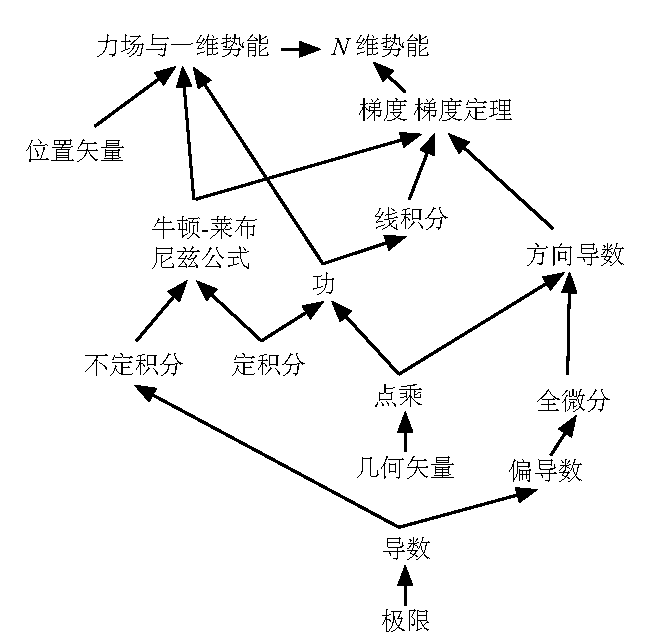
\includegraphics[width=10cm]{./figures/flowchart_example.pdf}
\caption{由“预备知识”画出的知识树(目标词条为“力场\ 势能\upref{V}”)}\label{FrontMatters_fig1}
\end{figure}

为了克服上述困难,百科采用以下形式:
\begin{enumerate}
\item 将知识点划分为词条, 且在每个词条中列出学习该词条前需要先学习哪些词条. 这样相当于建立了一个知识树(如\autoref{FrontMatters_fig1}). 项目网站 \href{https://wuli.wiki}{wuli.wiki} 上可以自动生成任意目标词条的知识树.
\item 采用词条分级,把同一个话题以不同深度,严谨度和适用范围等划分成若干个等级的同名词条.这样读者可以选择螺旋式学习(例如初中,高中,大学物理中所学的话题几乎相同,但程度不同).暂定初级词条从科普开始,尽量少使用数学.随着词条级别升高,会使用适用范围更广的定义,更严谨的表述和更抽象的数学等.
\end{enumerate}

\subsection{词条}
百科内容繁多,不同词条的重要性相去甚远,不建议初学者按照词条的排列顺序依次学习,而是应该以初级词条给出的主线来学习,再根据兴趣和需要阅读其余词条.

理论上来说,读者可以直接跳到最感兴的词条,如果“预备知识”中列出的词条都已经掌握,就可以开始学习该词条,否则就先掌握“预备知识”中的词条.如果“预备知识”出现在词条开始,则必须先掌握,如果出现在正文中,则只有阅读该部分时需要掌握.如果正文中引用了没有出现在“预备知识”中的内容,则读者可自行决定是否阅读.

为了便于书内的跳查,词条之间进行了大量的交叉引用,例如“导数简介\upref{Der}” 右上角中括号中的数字代表被引用词条的页码. 由于每个词条的公式编号都从 1 开始, 引用其他词条中的公式有时会用类似“\autoref{Der_eq2}~\upref{Der}” 的格式, 右上角的方括号中是公式所在词条的起始页码. 在本书的 PDF 电子版中,点击该页码即可自动跳转到对应的页面.在电脑上阅读,推荐使用 Adobe Reader 阅读器,在苹果\textsuperscript{\textregistered} 的 iOS 设备上推荐使用 GoodReader 应用( 两个软件都可以在不同的面板中打开同一本书的不同页码). 在 Adobe Reader 中,使用快捷键组合 “Alt +左箭头” 即可返回跳查前的位置,在移动设备的阅读软件中通常也有相应的返回按钮. 由于本书的电子版是原生 PDF(区别于扫描版), 还具有占用设备存储空间小, 便于分享, 便于查找关键字等种种优势.

%\subsection{5.本书符号约定}
%本书尽量使用物理学教科书中最常使用的符号,列出如下
%用粗体表示矢量,如 $\bvec F = m \bvec a$,用非粗体表示标量或矢量的模长,如 $\abs{\bvec F} = F$.同样用粗体表示矩阵,粗体上方加“$\^$”表示算符
% 未完成


% 物理学专业介绍 % 特别强调理科和工科的区别,介绍物理本科物理一般的学习内容
% 只学习最基础的规律,和模型,知识面广,但不复杂
% 由于太基础,会被认为“没有用”,离应用较远.
% 但物理又是其他理工科的基础
% 物理美在哪里? 更像是“艺术”,从几个最基本的假设出发,由数学推导出许多重要的结果.
% 本书遵循的理念:用尽可能少的公理,和尽可能简单的数学推导出结果,但有尽量保持严谨.
% 数学部分不可能做到像高等数学教材一样严谨,只求易懂且满足本书物理部分的使用.
% 均为本科物理专业教科书的标准内容,自己的内容或者超纲内容会在 “超纲内容” 部分中给出
 % 版权声明&关于本书
\setcounter{tocdepth}{1}
\tableofcontents % 生成目录
\mainmatter % 开始阿拉伯数字页码

\part{科普}
%=======================================
\chapter{经典力学}
%---------------------------------------
\entry{经典力学及其他物理理论}{MecThe}
\entry{经典力学}{CM0}
% \entry{动量和能量}{CM1} % 未完成
% \entry{角动量}{CM2} % 未完成

\chapter{电动力学}
%---------------------------------------
\entry{电动力学}{EM0}
\entry{静电的基本规律和性质}{EM1}
\entry{荷质比的测定}{Charge}
\entry{右手定则}{RHRul}
% \entry{电流产生磁场}{CurMag}
% \entry{楞次定律}{Lenz}

\chapter{量子力学}
%---------------------------------------
\entry{原子的观念}{AtomId}
\entry{从天球的音乐到玻尔模型}{ClBohr}
\entry{量子力学}{QM0}

\chapter{其他}
%---------------------------------------
\entry{天文学常识}{Astro}

\part{微积分}
%=======================================
\chapter{基础}
\entry{公理系统}{axioms}
\entry{集合}{Set}
\entry{整数}{intger}
\entry{映射}{map}
\entry{函数}{functi}
\entry{无穷的概念}{infty}
\entry{阶乘}{factor}
\entry{组合}{combin}
\entry{二项式定理}{BiNor}
\entry{二项式定理(非整数幂)}{BiNorR}
\entry{直线和平面的交点}{LPint}
\entry{等比数列}{GeoPrg}
\entry{三角恒等式}{TriEqv}
\entry{双曲函数}{TrigH}
\entry{sinc 函数}{sinc}
\entry{充分必要条件}{SufCnd}
\entry{四象限 Arctan 函数}{Arctan}
\entry{极坐标系}{Polar}
\entry{阿基米德螺线}{ArcSpl}
\entry{柱坐标系}{Cylin}
\entry{球坐标系}{Sph}
\entry{一元函数的对称与周期性}{shenry}
\entry{球坐标与直角坐标的转换}{SphCar}
\entry{圆锥曲线的极坐标方程}{Cone}
\entry{椭圆的三种定义}{Elips3}
\entry{双曲线的三种定义}{Hypb3}
\entry{抛物线的三种定义}{Para3}
\entry{圆锥曲线的光学性质}{ConOpt}
\entry{复数}{CplxNo}
\entry{复变函数}{Cplx}
\entry{幂函数(复数)}{CPow}
\entry{指数函数(复数)}{CExp}
\entry{三角函数(复数)}{CTrig}
\entry{复变函数的导数\ 柯西—黎曼条件}{CauRie}
\entry{复变函数的积分}{CpxInt}
\entry{柯西积分定理}{CauGou}
\entry{立体角}{SolAng}

\chapter{一元微积分}
%---------------------------------------
\entry{微积分导航}{Calc}
\entry{极限}{Lim}
\entry{小角正弦极限}{LimArc}
\entry{自然对数底}{E}
\entry{切线与割线}{TanL}
\entry{函数的连续性}{contin}
\entry{导数}{Der}
\entry{求导法则}{DerRul}
\entry{反函数求导}{InvDer}
\entry{基本初等函数的导数}{FunDer}
\entry{高阶导数}{HigDer}
\entry{莱布尼兹公式}{LeiEqu}
\entry{导数与函数极值}{DerMax}
\entry{用极值点确定函数图像}{DerImg}
\entry{一元函数的微分}{Diff}
\entry{复合函数求导\ 链式法则}{ChainR}
\entry{曲率\ 曲率半径(平面)}{curvat}
\entry{泰勒级数}{Taylor}
\entry{导数与差分}{DerDif}
\entry{不定积分}{Int}
\entry{换元积分法}{IntCV}
\entry{分部积分法}{IntBP}
\entry{积分表}{ITable}
\entry{定积分}{DefInt}
\entry{牛顿—莱布尼兹公式}{NLeib}
\entry{幂级数}{anal}
\entry{柯西—阿达玛公式}{CHF}
\entry{极坐标中的曲线方程}{PolCrd}
\entry{曲线的长度}{CurLen}
\entry{函数的算符}{DifOp}
\entry{常微分方程}{ODE}
\entry{一阶线性微分方程}{ODE1}
\entry{二阶常系数齐次微分方程}{Ode2}
\entry{一维齐次亥姆霍兹方程}{HmhzEq}
\entry{二阶常系数非齐次微分方程}{Ode2N}
\entry{正交函数系}{Fbasis}
\entry{傅里叶级数(三角)}{FSTri}
\entry{傅里叶级数(指数)}{FSExp}
\entry{狄拉克 delta 函数}{Delta}
\entry{狄拉克 delta 函数的正交归一性}{DeltOr}
\entry{傅里叶变换(三角)}{FTTri}
\entry{傅里叶变换(指数)}{FTExp}
\entry{拉普拉斯变换}{LapTra}
\entry{拉普拉斯变换的性质}{ProLap}
\entry{Gamma 函数}{Gamma}
\entry{渐近展开}{Asympt}
\entry{拉普拉斯方法}{LapAsm}

\chapter{多元微积分与矢量分析}
%---------------------------------------
\entry{偏导数}{ParDer}
\entry{最小二乘法}{LstSqr}
\entry{全微分}{TDiff}
\entry{复合函数的偏导\ 链式法则}{PChain}
\entry{全导数}{TotDer}
\entry{矢量的导数\ 求导法则}{DerV}
\entry{偏微分算符}{ParOp}
\entry{一元矢量函数的积分}{IntV}
\entry{方向导数}{DerDir}
\entry{二元函数的极值}{F2Exm}
\entry{重积分}{IntN}
\entry{极坐标系中单位矢量的偏导}{DPol1}
\entry{正交曲线坐标系}{CurCor}
\entry{多元函数的傅里叶级数}{NdFuri}
\entry{曲线坐标系中的重积分}{CrIntN}
\entry{矢量场}{Vfield}
\entry{线积分}{IntL}
\entry{曲面积分\ 通量}{SurInt}
\entry{证明闭合曲面的法向量面积分为零}{CSI0}
\entry{矢量算符}{VecOp}
\entry{拉普拉斯算符}{Laplac}
\entry{一种矢量算符的运算方法}{MyNab}
\entry{梯度\ 梯度定理}{Grad}
\entry{散度\ 散度定理}{Divgnc}
\entry{旋度}{Curl}
\entry{斯托克斯定理}{Stokes}
\entry{调和场}{HarmF}
\entry{矢量分析总结}{VecAnl}
\entry{亥姆霍兹分解}{HelDe}
\entry{拉格朗日乘数法}{LagMul}
\entry{一阶线性常微分方程组}{ODEsys}
\entry{齐次函数的欧拉定理}{Homeul}
\entry{多元泰勒展开}{NDtalr}
\entry{雅可比行列式}{JcbDet}
\entry{高斯积分}{GsInt}
\entry{多维球体的体积}{NSphV}
\entry{多元函数积分和宇称}{IntPry}

\part{线性代数}
\chapter{线性代数 1}
%---------------------------------------
\entry{线性代数导航}{Vector}
\entry{几何矢量}{GVec}
\entry{矢量内积}{Dot}
\entry{正交归一基底}{OrNrB}
\entry{施密特正交归一化}{SmdtOt}
\entry{矩阵}{Mat}
\entry{行列式}{Deter}
\entry{矢量叉乘}{Cross}
\entry{矢量叉乘分配律的几何证明}{CrossP}
\entry{叉乘的矩阵形式}{CrosMt}
\entry{连续叉乘的化简}{TriCro}
\entry{高斯消元法解线性方程组}{GAUSS}
\entry{线性相关\ 线性无关}{LinDep}
\entry{克莱姆法则}{Cramer}
\entry{三矢量的混合积}{TriVM}
\entry{平面旋转变换}{Rot2DT}
\entry{线性映射和线性变换}{LinMap}
\entry{线性映射的坐标表示}{LTrans}
\entry{逆矩阵}{InvMat}
\entry{平面旋转矩阵}{Rot2D}
\entry{三维旋转矩阵}{Rot3D}
\entry{过渡矩阵}{TransM}
\entry{绕轴旋转矩阵}{RotA}
\entry{旋转矩阵的导数}{RotDer}
\entry{厄米矩阵}{HerMat}
\entry{矩阵的本征方程}{MatEig}
\entry{对称矩阵的本征问题}{SymEig}
\entry{厄米矩阵的本征问题}{HerEig}
\entry{相似变换和相似矩阵}{MatSim}
\entry{矩阵的迹}{trace}

\chapter{线性代数 2}
%---------------------------------------
\entry{矢量空间}{LSpace}
\entry{对偶空间}{DualSp}
\entry{张成空间}{VecSpn}
\entry{矢量空间的表示}{VecRep}
\entry{内积}{InerPd}
\entry{狄拉克符号}{braket}
\entry{线性相关\ 线性无关}{LinInd}
\entry{子空间}{SubSpc}
\entry{直和}{DirSum}
\entry{对易算符}{Commu}
\entry{代数矢量}{NumVec}
\entry{矩阵与线性映射}{MatLS} % 未完成:把 MatSpc 合并到这里
\entry{正交子空间}{OrthSp}
\entry{矩阵的秩}{MatRnk}
\entry{证明矩阵行秩等于列秩}{RCrank}
% 未完成: 线性变换与矢量空间
\entry{线性方程组与矢量空间}{LinEq}
\entry{酉矩阵}{UniMat}
\entry{超定线性方程组}{OvrDet}
\entry{傅里叶变换与矢量空间}{FTvec}
\entry{海森矩阵}{Hesian}
\entry{四元数与旋转矩阵}{QuatN}

\chapter{张量代数}
%-------------------------------------------
\entry{张量积空间}{DirPro}
\entry{张量}{Tensor}
\entry{爱因斯坦求和约定}{EinSum}
\entry{张量的坐标变换}{TrTnsr}




\part{抽象代数}
%=======================================
\chapter{群论}
%---------------------------------------
\entry{群}{Group}
\entry{子群}{Group1}
\entry{陪集和同余}{coset}
\entry{正规子群}{NormSG}
\entry{群同态}{Group2}
\entry{群作用}{Group3}
\entry{商空间}{QuoSpa}
\entry{群的表示}{GrpRep}
\entry{自由群}{FreGrp}
\entry{群的自由积}{FrePrd}
\entry{群论中的证明和习题解答}{GroupP}

\chapter{环论}
%---------------------------------------
\entry{环}{Ring}
\entry{环的理想和商环}{Ideal}


\chapter{域论}
%---------------------------------------
\entry{域}{field}
\entry{域上的代数}{AlgFie}
\entry{四元数}{Quat}

\part{拓扑学}
%=====================================
\chapter{点集拓扑}
%-------------------------------------
\entry{拓扑空间}{Topol}
\entry{点集的内部、外部和边界}{Topo0}
\entry{连续映射和同胚}{Topo1}
\entry{紧致性}{Topo2}
\entry{连通性}{Topo3}
\entry{道路连通性}{Topo4}
\entry{分离性}{Topo5}
\entry{乘积拓扑}{Topo6}
\entry{商拓扑}{Topo7}
\entry{映射空间}{Topo8}
\entry{空间偶和带基点空间}{Topo9}
\entry{拓扑群}{TopGrp}

\chapter{同伦论}
%-------------------------------------
\entry{映射的同伦和空间的同伦}{HomT1}
\entry{可缩空间}{HomT2}
\entry{基本群}{HomT3}
\entry{高阶同伦群}{HomT4}
\entry{球面的同伦群}{SphHmt}
\entry{覆叠空间}{CovTop}
\entry{基本群的计算}{HomT5}


% by Jier:微分几何应该适合放在拓扑学后头,有点集拓扑和群论知识就可以讲得足够深入了;李代数的引入可能得两条路同时走,“直接从代数引入”和“从流形到李群到李代数的步步抽象”两种方式.
%======================================
\part{微分几何}
%=======================================
\chapter{欧几里得空间}
%-------------------------------------
\entry{光滑映射}{SmthM}
\entry{切空间(欧几里得空间)}{tgSpaE}

\chapter{流形}
%-------------------------------------
\entry{流形}{Manif}
\entry{子流形}{SubMnf}
\entry{流形上的切空间}{tgSpa}
\entry{抽象指标}{AbsInd}
\entry{切丛}{TanBun}
\entry{余切丛}{CotBun}
\entry{流形上的张量场}{TenMan}
\entry{向量丛}{VecBun}
\entry{切向量场}{Vec}
\entry{向量场的流}{VecFlo}
\entry{微分形式}{DiForm}
\entry{外微分}{ExtDif}
\entry{闭形式与恰当形式}{CloExa}
\entry{费罗贝尼乌斯定理}{FrobTh}

\chapter{联络}
%-------------------------------------
\entry{联络 (向量丛)}{VecCon}
\entry{曲率 (向量丛)}{VecCur}
\entry{平行性 (向量丛)}{VecPar}
\entry{和乐群(向量丛)}{VecHol}

\chapter{黎曼几何}
%-------------------------------------
\entry{黎曼度量与伪黎曼度量}{RiMetr}
\entry{Levi-Civita 联络}{LeCi}
\entry{测地线}{geodes}


\part{概率与统计}
%=======================================
\chapter{基础}
\entry{随机变量\ 概率分布函数}{RandF}
\entry{随机变量的变换}{RandCV}
\entry{多变量分布函数}{MulPdf}
\entry{高斯分布(正态分布)}{GausPD}
\entry{二项分布}{BiDist}
\entry{中心极限定理}{CLT}
\entry{二维随机走动}{RW2D}
\entry{平均值的不确定度}{MeanS}

\part{偏微分方程和特殊函数}
%=======================================
\chapter{基础}
%---------------------------------------
\entry{分离变量法}{SepVar}
\entry{拉普拉斯方程}{LapEq}
\entry{柱坐标系中的拉普拉斯方程}{CylLap}
\entry{球坐标系中的梯度散度旋度及拉普拉斯算符}{SphNab}
\entry{球坐标系中的拉普拉斯方程}{SphLap}
\entry{泊松方程}{PoiEqu}
\entry{球坐标系中的亥姆霍兹方程}{SphHHz}
\entry{勒让德多项式}{Legen}
\entry{连带勒让德多项式}{AsLgdr}
\entry{贝赛尔函数}{Bessel}
\entry{球贝塞尔函数}{SphBsl}
\entry{球谐函数}{SphHar}
\entry{球谐函数表}{YlmTab}
\entry{Wigner D 矩阵}{WigDmt}
\entry{平面波的正交归一}{PwOrNr}
\entry{平面波的球谐展开}{Pl2Ylm}
\entry{球谐波的归一化}{FrNorm}
\entry{分离变量法与张量积空间}{SVarDP}
\entry{广义球谐函数}{GenYlm}
\entry{误差函数}{Erf}
\entry{虚误差函数}{Erfi}
\entry{超几何函数}{HypGeo}
\entry{椭圆积分}{EliInt}
\entry{库仑函数}{CulmF}

\part{数学分析}
%=======================================
\chapter{基础}
\entry{集合的极限}{SetLim}
\entry{度量空间}{Metric}
\entry{范数}{NormV}
\entry{里斯引理(赋范空间)}{RiLem}
\entry{投影算符}{projOp}
\entry{柯西—施瓦茨不等式}{CSNeq}
\entry{巴拿赫空间}{banach}
\entry{巴拿赫定理}{BanThm}
\entry{一致收敛}{UniCnv}
\entry{数学分析笔记}{AnalNt}
\entry{黎曼积分与勒贝格积分}{Rieman}

\part{泛函分析}
%====================================
\chapter{笔记}
\entry{希尔伯特空间}{Hilber}
\entry{泛函分析笔记1}{FnalNt}
\entry{泛函分析笔记2}{FnalN2}
\entry{泛函分析笔记3}{FnalN3}
\entry{泛函分析笔记4}{FnalN4}
\entry{泛函分析笔记5}{FnalN5}

\chapter{其他}
%---------------------------------------
\entry{堆放排列组合}{StackC}
\entry{范德蒙恒等式}{ChExpn}
\entry{解三棱锥顶角}{PrmSol}
\entry{足球顶点坐标的计算}{FootBl}
\entry{CG 系数}{SphCup}
\entry{Wigner 3j 符号}{ThreeJ}
\entry{Wigner 6j 符号}{SixJ}
\entry{Wigner 9j 符号}{NineJ}
\entry{二元关系}{Relat}
\entry{群论笔记}{GroupN}
\entry{范畴论}{Cat}
\entry{余元公式}{Gama1}

\part{经典力学}
%=======================================
\chapter{质点运动学}
%---------------------------------------
\entry{物理量和单位转换}{Units}
\entry{无量纲的物理公式}{NoUnit}
\entry{位置矢量\ 位移}{Disp}
\entry{速度\ 加速度(一维)}{VnA1}
\entry{速度\ 加速度}{VnA}
\entry{圆周运动的速度}{CMVD}
\entry{圆周运动的加速度}{CMAD}
\entry{匀加速运动}{ConstA}
\entry{匀速曲线运动}{PCuvMo}
% \entry{变速曲线运动}{VarCur}
\entry{极坐标中的速度和加速度}{PolA}
\entry{速度的坐标系变换}{Vtrans}
\entry{加速度的坐标系变换}{AccTra}

\chapter{质点动力学}
%---------------------------------------
\entry{力的分解与合成}{Fdecom}
\entry{牛顿运动定律\ 惯性系}{New3}
\entry{圆周运动的向心力}{CentrF}
\entry{重力\ 重量}{Weight}
\entry{功\ 功率}{Fwork}
\entry{动能\ 动能定理(单个质点)}{KELaw1}
\entry{力场\ 势能}{V}
\entry{机械能守恒(单个质点)}{ECnst}
\entry{动量\ 动量定理(单个质点)}{PLaw1}
\entry{角动量\ 角动量定理\ 角动量守恒(单个质点)}{AMLaw1}
\entry{简谐振子}{SHO}
\entry{受阻落体}{RFall}
\entry{单摆}{Pend}
\entry{傅科摆}{Fouclt}
\entry{惯性力}{Iner}
\entry{离心力}{Centri}
\entry{科里奥利力}{Corio}
\entry{地球表面的科里奥利力}{ErthCf}

\chapter{质点系与刚体}
%---------------------------------------
\entry{自由度}{DoF}
\entry{质点系}{PSys}
\entry{质心\ 质心系}{CM}
\entry{质点系的动量}{SysMom}
\entry{刚体}{RigBd}
\entry{轻杆模型}{rod}
\entry{动量定理\ 动量守恒}{PLaw}
\entry{质点系的动能\ 柯尼希定理}{Konig}
\entry{力矩}{Torque}
\entry{刚体的静力平衡}{RBSt}
\entry{角动量}{AngMom}
\entry{角动量定理\ 角动量守恒}{AMLaw}
\entry{二体系统}{TwoBD}
\entry{二体碰撞}{TwoCld}
\entry{刚体的绕轴转动\ 转动惯量}{RigRot}
\entry{平行轴定理与垂直轴定理}{MIthm}
\entry{常见几何体的转动惯量}{ExMI}
\entry{刚体的平面运动方程}{RBEM}
\entry{惯性张量}{ITensr}
\entry{瞬时转轴}{InsAx}
\entry{刚体绕轴转动 2}{RBrot2}
\entry{刚体的动能定理}{RBKE}
\entry{刚体的运动方程}{RBEqM}
\entry{刚体运动方程(四元数)}{RBEMQt}

\chapter{软体和流体}
%---------------------------------------
\entry{绳的法向压力}{RopeFP}
\entry{流密度}{CrnDen}
\entry{浮力}{Buoy}
\entry{伯努利方程}{Bernul}

\chapter{振动与波动}
%---------------------------------------
\entry{振动的指数形式}{VbExp}
\entry{能量法解谐振动问题}{EnerVi}
\entry{拍频}{beatno}
\entry{受阻简谐振子}{SHOf}
\entry{简谐振子的品质因数}{SHOq}
\entry{简谐振子受迫运动}{SHOfF}
\entry{共振}{ResoN}
\entry{平面波}{PWave}
\entry{波包}{WvPck}
\entry{高斯波包}{GausPk}
\entry{多普勒效应(一维匀速)}{Dople1}
\entry{多普勒效应}{Dopler}
\entry{一维波动方程}{WEq1D}
% 未完成 边界条件 (两条密度不同的绳子)
\entry{二维波动方程}{Wv2D}
\entry{波的能量}{WaEner}
\entry{波的强度}{WaInte}
\entry{冲击波}{ShoWav}

\chapter{中心力场问题}
%---------------------------------------
\entry{万有引力\ 引力势能}{Gravty}
\entry{壳层定理}{SphF}
\entry{中心力场问题}{CenFrc}
\entry{开普勒问题}{CelBd}
\entry{开普勒三定律}{Keple}
\entry{拉普拉斯—龙格—楞次矢量}{LRLvec}
\entry{轨道方程\ 比耐公式}{Binet}
\entry{开普勒第一定律的证明}{Keple1}
\entry{开普勒第二和第三定律的证明}{Keple2}
\entry{反开普勒问题}{InvKep}
\entry{散射}{Scater}
\entry{卢瑟福散射}{RuthSc}
\entry{闭合轨道的条件}{ClsOrb}

\chapter{分析力学}
%---------------------------------------
\entry{拉格朗日方程}{Lagrng}
\entry{拉氏方程和极值问题}{LagPrb}
\entry{贝尔特拉米等式}{Beltra}
\entry{最速降线问题}{Brachi}
\entry{单摆(大摆角)}{SinPen}
\entry{双摆和三摆}{Pendu3}
\entry{达朗贝尔定理}{dAlbt}
\entry{最小作用量 哈密顿原理}{HamPrn}
\entry{运动积分}{motint}
\entry{勒让德变换}{TrLgdr}
\entry{哈密顿正则方程}{HamCan}
\entry{分析力学笔记}{ClsMec}

\chapter{轨道力学}
%---------------------------------------
\entry{二体问题综述}{ConDB}
\entry{轨道参数\ 时间变量}{OribP}
\entry{限制性三体问题}{TriLim}
\entry{雅可比常量}{JConst}
\entry{拉格朗日点}{LPoint}


\part{光学}
%=======================================
\chapter{几何光学}
%---------------------------------------
\entry{惠更斯原理}{Huygen}
\entry{光的折射\ 斯涅尔定律}{Snel}
\entry{薄透镜}{ThnLen}

\chapter{波动光学}
%---------------------------------------
\entry{可见光谱}{VisSpt}
\entry{双缝干涉中一个重要极限}{SltLim}
\entry{杨氏双缝干涉实验}{Young}
\entry{劳埃德镜实验}{Lloyd}
\entry{普通光源的发光机理}{LumiMe}
\entry{单色光}{MonoLi}
\entry{高斯光束}{GausBm}

\part{电动力学}
%=======================================
\chapter{基础}
%---------------------------------------
\entry{电流}{I}
\entry{电流密度}{Idens}
\entry{库仑定律}{ClbFrc}
\entry{电场}{Efield}
\entry{电势\ 电势能}{QEng}
\entry{电偶极子}{eleDpl}
\entry{电偶极子2}{eleDP2}
\entry{导体}{Cndctr}
\entry{电压}{Voltag}
\entry{电容}{Cpctor}
\entry{电介质}{Dielec}
\entry{电极化强度}{ElecPo}
\entry{电极化强度与极化电荷的关系}{ElePAP}
\entry{极化电流}{PolCur}
\entry{介质中的静电场}{EFIDE}
\entry{电阻\ 欧姆定律}{Resist}
\entry{电感}{Induct}
\entry{电场的高斯定理}{EGauss}
\entry{电场的高斯定理证明}{EGausP}
\entry{电场的能量}{EEng}
\entry{LC 振荡电路}{LC}
\entry{力电振动类比}{MeElec}
\entry{LC 受迫振荡电路}{EleRes}
\entry{比奥萨伐尔定律}{BioSav}
\entry{安培环路定理}{AmpLaw}
\entry{洛伦兹力}{Lorenz}
\entry{磁场的能量}{BEng}
\entry{磁通量}{BFlux}
\entry{安培力}{FAmp}
\entry{磁矩}{MagMom}
\entry{磁场中闭合电流的合力}{EBLoop}
\entry{磁场中闭合电流的力矩}{EBTorq}
\entry{法拉第电磁感应定律}{FaraEB}
\entry{分子电流和分子磁矩}{MoMaMo}
\entry{磁介质}{MagMat}
\entry{磁化强度}{MaInte}
\entry{顺磁质的磁化}{ParaMa}
\entry{有磁介质时的安培环路定理}{MaAmpe}
\entry{电路}{Circ}
\entry{基尔霍夫电路定律}{Kirch}
\entry{惠斯通电桥}{WheBrg}

\chapter{电动力学 2}
%---------------------------------------
\entry{电荷守恒\ 电流连续性方程}{ChgCsv}
\entry{电多极展开}{EMulPo}
\entry{电磁场标势和矢势}{EMPot}
\entry{磁标势}{elecdy}
\entry{磁多极矩}{edy33}
\entry{规范变换}{Gauge}
\entry{洛伦兹规范}{LoGaug}
\entry{库仑规范}{Cgauge}
\entry{电磁场的能量守恒\ 坡印廷矢量}{EBS}
\entry{麦克斯韦方程组}{MWEq}
\entry{麦克斯韦方程组(介质)}{MWEq1}
\entry{非齐次亥姆霍兹方程\ 推迟势}{RetPot}
\entry{电场波动方程}{EWEq}
\entry{真空中的平面电磁波}{VcPlWv}
\entry{介质中的波动方程}{MedWF}
\entry{菲涅尔公式\ 布儒斯特角}{Fresnl}
\entry{盒中的电磁波}{EBBox}
\entry{电磁场的动量守恒\ 动量流密度张量}{EBP}
\entry{磁旋比\ 玻尔磁子}{BohMag}

\chapter{电动力学 3}
%---------------------------------------
\entry{电磁场的参考系变换}{EMRef}
\entry{拉格朗日电磁势}{EMLagP}
\entry{电磁场角动量分解}{EMAMSp}

\part{相对论}
%=======================================
\chapter{狭义相对论}
%---------------------------------------
\entry{狭义相对论的基本假设}{SpeRel}
\entry{事件与尺缩效应}{SRsmt}
\entry{时间的变换与钟慢效应}{SRtime}
\entry{洛伦兹变换}{SRLrtz}
\entry{斜坐标系}{ObSys}
\entry{斜坐标系表示洛伦兹变换}{SROb}
\entry{约化光速}{SRc}
\entry{洛伦兹变换的代数推导}{LornzT}
\entry{相对论速度变换}{RelVel}
\entry{相对论加速度变换}{SRAcc}
\entry{时空的四维表示}{SR4Rep}
\entry{闵可夫斯基空间}{MinSpa}
\entry{光的多普勒效应}{RelDop}
\entry{洛伦兹群}{qed1}


\chapter{相对论动力学}
%---------------------------------------
\entry{相对论动力学假设}{SRDyn}
\entry{尘埃云的能动张量}{SRFld}

\chapter{广义相对论}
%---------------------------------------
\entry{双生子佯谬}{Twins}



\part{量子力学}
%=======================================
% 未完成 讲讲为什么定态波函数一定是实数函数? 实数波函数为什么会有动量平均值为零?
% 未完成 x,p 不确定原理,一般的不确定原理, 高斯波包时取等号.
% 未完成 束缚态的一般性质: 节点数, 对称性 (偶势能的基态是偶函数), 简并性(一维情况不简并)

\chapter{量子力学 1}
%---------------------------------------
\entry{玻尔原子模型}{BohrMd}
\entry{原子单位制}{AU}
\entry{自然单位制}{NatUni}
\entry{指数衰减}{ExpDec}
\entry{精细结构常数}{FinStr}
\entry{量子力学与矩阵}{QMmat}
\entry{算符和本征问题}{QM1}
\entry{定态薛定谔方程}{SchEq}
\entry{薛定谔方程}{TDSE}
\entry{不确定原理}{Uncert}
\entry{多维空间中的量子力学}{QMndim}
\entry{一维高斯波包(量子)}{GausWP}
\entry{无限深势阱}{ISW}
\entry{升降算符}{RLop}
\entry{简谐振子(升降算符)}{QSHOop}
\entry{简谐振子升降算符归一化}{QSHOnr}
\entry{简谐振子(级数)}{QSHOxn}
\entry{有限深球势阱}{FiSph}
\entry{一维 delta 势能散射}{Dsc1D}
\entry{方势垒}{SqrPot}
\entry{拉比频率}{RabiF}
\entry{二维无限深势阱}{ISW2D}
\entry{平均值(量子力学)}{QMavg}
\entry{守恒量(量子力学)}{QMcons}
\entry{好量子数}{GoodQN}
\entry{薛定谔方程的分离变量法}{SEsep}
\entry{对易厄米算符与共同本征矢}{Commut}
\entry{类氢原子的约化质量}{HRMass}
\entry{概率流密度}{PrbJ}
\entry{算符的矩阵表示}{OpMat}
\entry{轨道角动量}{QOrbAM}
\entry{轨道角动量升降算符归一化}{QLNorm}
\entry{自旋角动量}{Spin}
\entry{自旋角动量矩阵}{spinMt}

\chapter{量子力学 2}
%---------------------------------------
\entry{算符的指数函数\ 波函数传播子}{OpExp}
\entry{平移算符}{tranOp}
\entry{旋转算符}{rotOp}
\entry{角动量加法(量子力学)}{AMAdd}
\entry{能量归一化}{EngNor}
\entry{氢原子基态的波函数}{HWF0}
\entry{球坐标和柱坐标中的定态薛定谔方程}{RadSE}
\entry{球坐标中的薛定谔方程}{RYTDSE}
\entry{量子力学中的变分法}{QMVar}
\entry{含时微扰理论}{TDPT}
\entry{几种含时微扰}{TDPEx}
\entry{含连续态的微扰理论}{PTCont}
\entry{量子散射}{ParWav}
\entry{波恩近似(散射)}{BornSc}
\entry{质心系中的多粒子问题}{SECM}
\entry{三维简谐振子(球坐标)}{SHOSph}
\entry{球面散射态与平面散射态的转换}{Scatt2}
\entry{库仑波函数}{CulmWf}
\entry{量子力学的基本假设}{QMPos}
\entry{带电粒子的薛定谔方程}{EMTDSE}
\entry{电磁场中的单粒子薛定谔方程}{QMEM}
\entry{电磁场中的类氢原子}{EMHydr}
\entry{氢原子电离截面}{HionCr}
\entry{Volkov 波函数}{Volkov}
\entry{氢原子的选择定则}{SelRul}
\entry{康普顿散射}{Comptn}
\entry{全同粒子}{IdPar}
\entry{密度矩阵}{denMat}
\entry{Hartree-Fork 方法}{HarFor}
\entry{多通道散射}{MulSct}
\entry{Adiabatic 笔记}{Adibat}
\entry{晶体衍射}{CrysDf}
\entry{超导唯象解释——伦敦方程}{edy34}

\chapter{量子力学与量子场论}
%---------------------------------------
\entry{前言}{QFIntro}
\entry{基本概念}{Basics}
\entry{全同粒子的统计}{IdParS}
\entry{近似理论:微扰}{AprPtr}
\entry{角动量}{QMAM}
% 第六章直接从 sakurai 翻译, 后面的一些内容非常零碎跳过
\entry{冷原子基本知识}{UCBas}
\entry{两个原子间的相互作用}{TwoAtF}
\entry{Feshbach 共振}{FeshRs}
\entry{BCS-BEC Crossover 的平均场描述}{BCSBEC}
\entry{BEC 超流}{BECSup}

\part{原子分子物理}
%=======================================
\chapter{原子}
%---------------------------------------
\entry{类氢原子的定态波函数}{HWF}
\entry{氢原子波函数分析}{Hanaly}
\entry{电子轨道与元素周期表}{Ptable}
\entry{能项符号}{TrmSym}
\entry{氢线(21厘米线)}{HydroL}
\entry{兰姆位移}{LambSh}
\entry{Keldysh 参数}{keldis}
\entry{FROG}{Frog}

\chapter{分子}
%---------------------------------------
\entry{双原子分子势能曲线}{dpecs}

\part{热力学和统计力学}
%=======================================
\chapter{热力学}
%---------------------------------------
\entry{气体分子对容器壁的压强}{MolPre}
\entry{理想气体状态方程}{PVnRT}
\entry{温度\ 温标}{tmp}
\entry{理想气体的内能}{IdgEng}
\entry{压强体积图}{PVgraf}
\entry{热平衡\ 热力学第零定律}{TherEq}
\entry{热传导定律}{Heatco}
\entry{热力学第一定律}{Th1Law}
\entry{等压过程}{EqPre}
\entry{等体过程}{EqVol}
\entry{等温过程}{EqTemp}
\entry{热容量}{ThCapa}
\entry{绝热过程}{Adiab}
\entry{熵}{Entrop}
\entry{准静态过程}{Quasta}
\entry{卡诺热机}{Carnot}
\entry{分子平均碰壁数}{AvgHit}
\entry{气体分子的速度分布}{VelPdf}
\entry{麦克斯韦—玻尔兹曼分布}{MxwBzm}
\entry{理想气体分压定律}{PartiP}
\entry{饱和蒸汽压}{VaporP}
\entry{黑体辐射定律}{BBdLaw}
\entry{维恩位移定律}{WienDs}
\entry{斯特藩—玻尔兹曼定律}{SteBol}

\chapter{统计力学}
%---------------------------------------
\entry{相空间}{PhSpace}
\entry{理想气体的状态密度(相空间)}{IdSDp}
\entry{理想气体单粒子能级密度}{IdED1}
\entry{理想气体(微正则系综法)}{IdNCE}
\entry{正则系宗法}{CEsb}
\entry{理想气体(正则系宗法)}{IdCE}
\entry{理想气体(巨正则系综法)}{IdMCE}
\entry{等间隔能级系统(正则系宗)}{EqCE}
\entry{巨正则系综法}{MCEsb}
\entry{量子气体(单能级巨正则系综法)}{QGs1ME}
\entry{量子气体(巨正则系宗)}{QGsME}
\entry{光子气体}{PhoGas}
\entry{理想气体的熵:纯微观分析}{IdeaS}
\entry{Ising 模型}{Ising}
\entry{统计力学公式}{StatEq}

\part{近代物理}
%=======================================
\chapter{高能物理}
%---------------------------------------
\entry{基本粒子}{BasPar}

\chapter{弦理论}
%---------------------------------------
\entry{引力量子化}{QuanGR}
\entry{弦论概述}{STover}
\entry{弦论的种类}{TYPEst}
\entry{BRST 量子化}{BRST}
\entry{RNS 超弦}{RNS}
% \chapter{经典弦 1}
%---------------------------------------
% \chapter{经典弦 2}
%---------------------------------------
% \chapter{弦量子化}
%---------------------------------------
% \chapter{共形场论 1}
%---------------------------------------
% \chapter{BRST 量子化}
%---------------------------------------
% \chapter{RNS 超弦}
%---------------------------------------
% \chapter{紧致化和T对偶}
%---------------------------------------
% \chapter{超弦理论\ 续}
%---------------------------------------
% \chapter{超弦理论\ 总结}
%---------------------------------------
% \chapter{第II型弦论}
%---------------------------------------
% \chapter{Heterotic 弦论}
%---------------------------------------
% \chapter{D-膜}
%---------------------------------------
% \chapter{黑洞}
%---------------------------------------
% \chapter{全息原理和AdS/CFT}
%---------------------------------------
% \chapter{弦理论和宇宙学}

\chapter{宇宙学}
%---------------------------------------
\entry{宇宙的演化}{UniEvo}

\chapter{宇宙学扰动}
\entry{标量扰动}{ScaPT}
\entry{张量扰动}{TenPT}

\chapter{引力波}
\entry{引力波的几何描述}{Geomet}
\entry{TT 规范}{TTGaug}
\entry{引力波和测试质量的相互作用}{intera}

\part{科学计算}
%=======================================
\chapter{Matlab 简介}
% 未完成 Mathematica
% 未完成 Wolfram Alpha
%---------------------------------------
\entry{计算物理导航}{NumPhy}
\entry{Matlab 简介}{Matlab}
\entry{Matlab 的变量与矩阵}{MatVar}
\entry{Matlab 的判断与循环}{MIfFor}
\entry{Matlab 的函数}{MatFun}
\entry{Matlab 画图}{MatPlt}
\entry{Matlab 的程序调试及其他功能}{MatOtr}

\chapter{Python 简介}
%---------------------------------------
\entry{Python 简介}{Python}
\entry{Python 基本变量类型}{PyType}
\entry{Python 数据类型}{PyData}
\entry{Numpy 库}{numpy}
\entry{Python 字符串处理}{PyStr}
\entry{Python 文件读写}{PyFile}
\entry{Python 判断与循环}{PyIfFr}
\entry{Python 函数}{PyFunc}
\entry{Python 画图}{PyPlot}
\entry{Python 的类}{PyClas}
\entry{Python 模块}{PyMod}
\entry{SciPy 数值微分与积分}{SciPy}
\entry{SciPy 最小二乘法}{PyFit}

\chapter{Linux 简介}
%---------------------------------------
\entry{Linux 基础}{Linux}
\entry{在 Linux 上编译 C/C++ 程序}{linCpp}
\entry{Makefile 简介}{Make0}
\entry{Makefile 笔记}{Make}

\chapter{C++ 简介}
%---------------------------------------
\entry{C++ 基础}{Cpp0}
\entry{C++ 的整数}{cppInt}
\entry{C/C++ 多文件编译笔记}{cppFil}
\entry{调试 C++ 程序}{gdbcpp}
% \entry{SLISC0 库简介}{SLISC}
\entry{BLAS 简介}{BLAS}
\entry{矩阵的数据结构}{MatSto}
\entry{带对角矩阵(BLAS)}{BanDmt}
\entry{GNU Scientific Library}{GSL}
\entry{简单的矢量和矩阵类}{SLSvec}
\entry{C++ 中的 SFINAE 技巧}{SFINAE}

\chapter{其他}
%---------------------------------------
\entry{文本文件与字符编码}{encode}
\entry{正则表达式}{regex}
\entry{LaTeX 结构简介}{latxIn}
\entry{校验和}{chkSum}
\entry{GitHub Desktop 的简单使用}{GitHub}
\entry{cuBLAS 库}{cublas}
\entry{Julia 分形}{julias}
% \entry{用百度网盘安全高效地备份文件}{PanBak}

\chapter{数值验证及常用算法}
%---------------------------------------
\entry{二项式定理(非整数幂)的数值验证}{BiNorM}
\entry{二分法}{Bisec}
\entry{多区间二分法}{MBisec}
\entry{冒泡法}{Bubble}
\entry{高斯消元法程序}{GauEli}
\entry{Nelder-Mead 算法}{NelMea}
\entry{最小二乘法的数值计算}{CurFit}
\entry{数值积分(梯形法)}{NumInt}
\entry{稀疏矩阵}{SprMat}
\entry{函数求值}{SpcFun}
\entry{离散傅里叶变换}{DFT}
\entry{离散正弦变换}{DST}

\chapter{计算机图形学}
%---------------------------------------
\entry{图像坐标系}{imgFrm}
\entry{三维投影}{proj3D}
\entry{相机模型}{CamMdl}
\entry{由图像坐标计算射线}{mn2lin}
\entry{计算 3D 艺术画}{art3D}
\entry{相机的定位}{CamLoc}
\entry{长方形相机定位法}{RecCam}

\chapter{微分方程数值解}
%---------------------------------------
\entry{简谐振子受迫运动的简单数值计算}{SHOFN}
\entry{天体运动的简单数值计算}{KPNum0}
\entry{常微分方程(组)的数值解}{OdeNum}
\entry{中点法解常微分方程(组)}{OdeMid}
\entry{四阶龙格库塔法}{OdeRK4}
\entry{刚体转动数值模拟}{RBRNum}

\chapter{偏微分方程数值解}
%---------------------------------------
\entry{一维波动方程的数值解}{W1dNum}

\chapter{一维薛定谔方程数值解}
%---------------------------------------
\entry{一维势能束缚态数值解(试射法)}{BndSho}
\entry{无限深势阱中的高斯波包}{wvISW}

\chapter{氢原子薛定谔方程数值解}
%---------------------------------------
\entry{球谐函数数值计算}{YlmNum}
\entry{Crank-Nicolson 算法(一维)}{CraNic}
\entry{Gauss-Lobatto 积分}{GLquad}
\entry{FEDVR 算法}{FEDVR}
\entry{Lanczos 算法}{Lanc}
\entry{指数格点}{ExpGrd}
\entry{虚时间法求基态波函数}{ImgT}
\entry{氢原子薛定谔方程数值解}{HyTDSE}
\entry{氢原子球坐标数值解 TDSE}{HTDSE}

\chapter{氦原子薛定谔方程数值解}
%---------------------------------------
\entry{氦原子数值解 TDSE 笔记}{HeTDSE}
\entry{氦原子波函数数值分析}{HeAnal}

\part{附录}
%=======================================
\chapter{附录}
%---------------------------------------
\entry{本书符号与规范}{Conven}
\entry{常见物理量}{PhyQty}
\entry{国际单位制}{SIunit}
\entry{物理学常数}{Consts}
\entry{国际单位制词头}{UniPre}
\entry{厘米—克—秒单位制}{CGS}
\entry{小时百科图标}{xwLogo}
\bibli
\end{document}
